Suszeptibilität lässt sich nicht direkt messen, beeinflusst allerdings die Induktivität einer
Spule nach Gl.\ref{eqspule}.
\begin{align}
&L_m=\mu_0 \frac{n^2 F}{l} + \chi \mu_0 \frac{n^2 Q}{l} \label{eqspule} \\
&F: Spulenquerschnitt, Q: Probenquerschnitt \nonumber
\end{align}
Ein Selektivverstärker filtert Frequenzen, so das Störspannungen zu einem großen Teil ausgeblendet 
werden können. Eine wichtige Eigenschaft dieses Bauteils ist dabei die Güte $Q$, welche beschreibt, 
wann das Verhältnis von $U_A$ zu $U_E$ auf $1/\sqrt{2}$ abgesunken ist.
\begin{align}
Q&=\frac{\nu_0}{\nu_+ - \nu_-} \label{eqn:engute}
\end{align}
	\begin{figure}[h]
		\begin{center}
		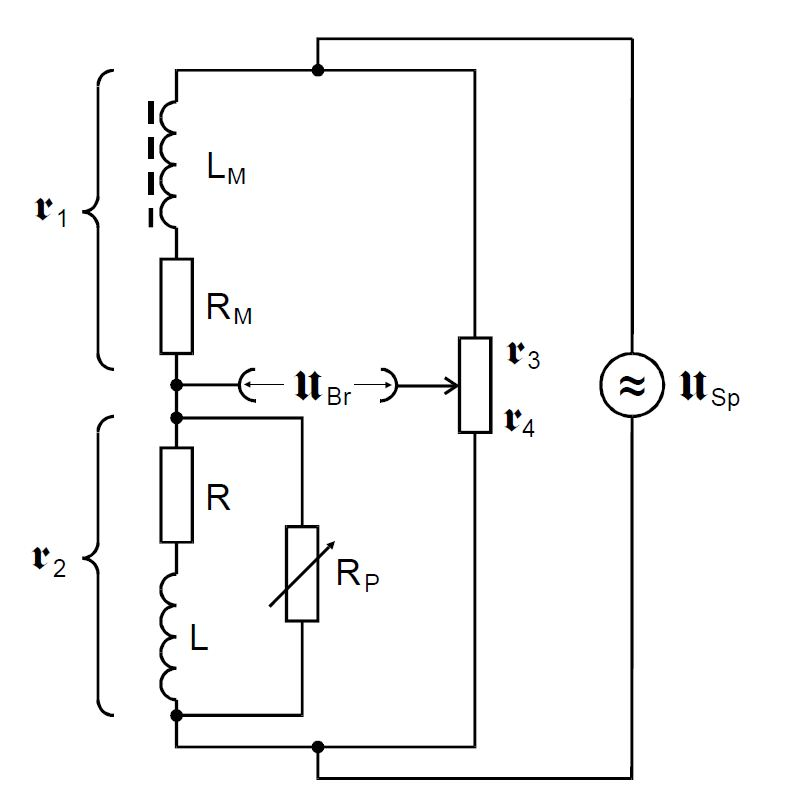
\includegraphics[scale=0.3]{picbrucke.jpg}
		\caption{Brückenschaltung mit Spulen$^{[1]}$}
		\label{picbrucke}
		\end{center}	
	\end{figure}
\FloatBarrier
Um Widerstände zu messen wird häufig eine Brückenschaltung (Abb.\ref{picbrucke}) verwendet. Diese beruht auf dem Prinzip 
Widerstandsverhältnisse zueinander zu messen. Die vier Widerstände, welche in zwei Reihenschaltungen
parallel geschaltet sind werden auf Null abgeglichen bevor der unbekannte Widerstand hinzu kommt. 
Wird als unbekannter Widerstand die bekannte Spule mit Materie gefüllt, so lassen sich folgende Gleichungen
herleiten.
\begin{align}
\chi(U_{Br})&=\frac{U_{Br}}{U_{Sp}}\frac{4l}{\omega \mu_0 n^2 Q} \sqrt{R^2 + \omega^2 (\mu_0 \frac{n^2}{l} F)^2} \label{eqn:chibrucke}\\
für \omega^2 L^2 \gg R^2 : \nonumber \\
\chi(U_{Br})&=4 \frac{F U_{Br}}{Q U_{Sp}} \label{eqchiu}\\
\chi(\Delta R)&=2 \frac{\Delta R F}{R_3 Q} \label{eqchir}
\end{align}
%\FloatBarrier
	\begin{figure}[h]
		\begin{center}
		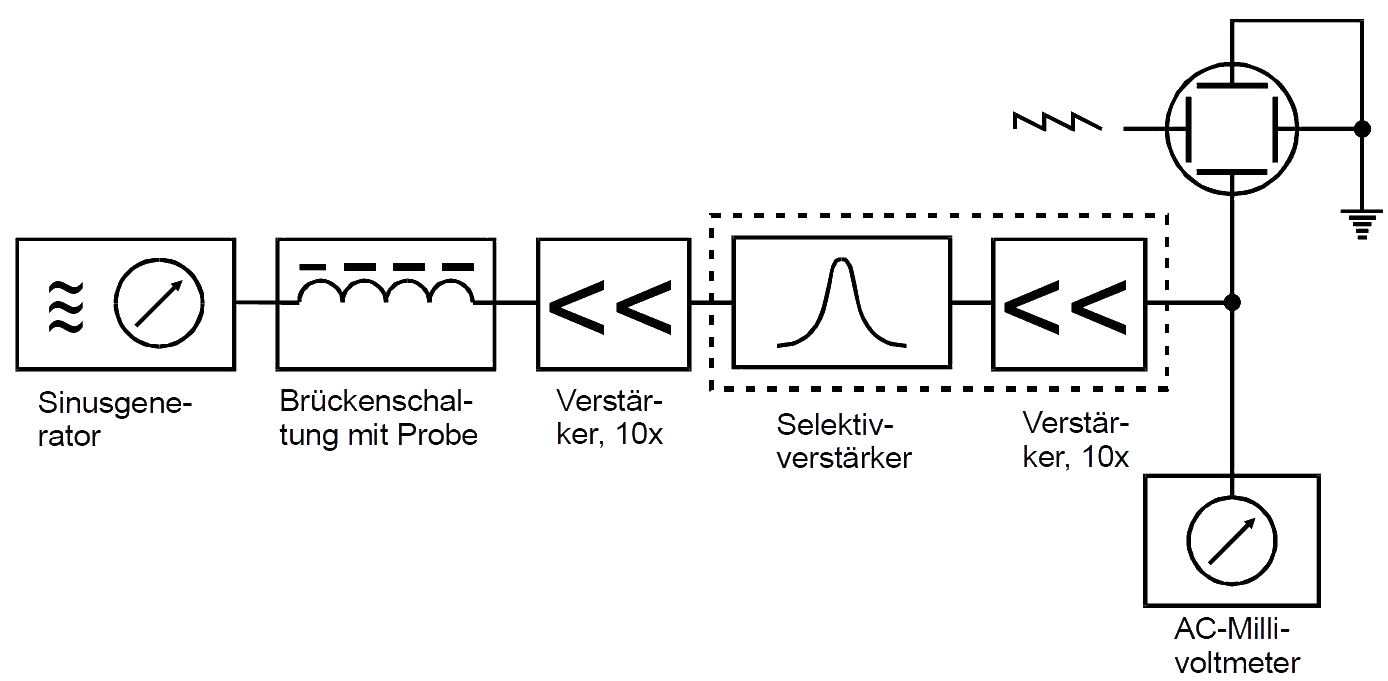
\includegraphics[scale=0.3]{picaufbau.jpg}
		\caption{Aufbau der Messanordnung$^{[1]}$}
		\label{picaufbau}
		\end{center}	
	\end{figure}
Die Messapparatur wurde wie in Abbildung \ref{picaufbau} aufgebaut. Zu Beginn wurde der Selektivverstärker
ausgekoppelt betrachtet um Werte für die Gütekurve aufzuzeichnen. Dabei wurde unter Frequenzvariation bei 
fester Eingangsspannung die Ausgangsspannung abgelesen. \\ 
Um die Verstärkung zu verifizieren wurde dann bei Durchlassfrequenz die selektivverstärkereigene zehnfach 
Verstärkung getestet, sowie die externe zehnfach Verstärkung überprüft.\\
Darauf folgend wurden die Elemente wieder eingekoppelt (Abb.\ref{picaufbau}) und es wurde mit einem anderen 
Sinusgenerator die Proben von $Nd_2O_3$,$Gd_2O_3$ und $Dy_2O_3$ untersucht. Dabei wurde die Brückenschaltung
jeweils zuerst auf Null abgeglichen, dann die Probe eingeführt und abermals auf Null abgeglichen.

